\documentclass[11pt,a4paper]{article}

\usepackage[margin=1.5cm]{geometry}
\usepackage[T1]{fontenc}
\usepackage{lmodern}
\usepackage{microtype}
\usepackage{amsmath}
\usepackage{graphicx}
\usepackage{booktabs}
\usepackage{tabularx}
\usepackage{longtable}
\usepackage{array}
\usepackage{xcolor}
\usepackage{enumitem}
\usepackage{float}
\usepackage[font=small,labelfont=bf,skip=4pt]{caption}
\usepackage[colorlinks=true,linkcolor=blue!50!black,urlcolor=blue!50!black]{hyperref}

\setlist{itemsep=1pt,topsep=3pt}
\setlength{\parskip}{5pt}
\setlength{\parindent}{0pt}
\setlength{\LTpre}{4pt}
\setlength{\LTpost}{2pt}
\renewcommand{\arraystretch}{1.15}
\newcolumntype{Y}{>{\raggedright\arraybackslash}X}
\newcolumntype{R}{>{\raggedleft\arraybackslash}X}
\newcolumntype{P}[1]{>{\raggedright\arraybackslash}p{\dimexpr#1\textwidth-2\tabcolsep\relax}}
\newcommand{\code}[1]{\texttt{\small #1}}

\title{\textbf{Chart Claim Verifier}}
\author{\begin{tabular}{ll}
Harsh Raj (2025202005) & \hspace{2em}Hritik Ranjan (2025202031) \\
Karan Thayat (2025202008) & \hspace{2em}Vikash Kumar (2025201012)\\ \end{tabular}\\ LMA Project 2026 Mid Submission\\ {\normalsize Code: \url{https://github.com/IIITH-2025-27/ReportLens}}}
\date{}

\begin{document}
\maketitle

\begin{abstract}
\noindent We are building a system that checks whether the numbers in a lab report match the report's own charts. Up to four tools read each value. The median is the estimate, and an error margin based on how much the tools disagree, scaled on charts with known values, decides whether the claim is accepted, flagged or passed to the TA. A planner picks the tools, and the system's only action is posting a flag. On 100 generated reports (1{,}000 claims) it decides 78.6\% of claims, is right on 96.8\% of those, and 3.0\% of its flags are wrong, against 36.1\% for the same VLM asked directly. Three results were weaker than expected: an uncalibrated margin did as well as the calibrated one, one test set had 9.4\% wrong flags, and fine-tuning improved reading but not wrong flags. Baseline B3, two experiments and a final untouched test set remain for 13 November.
\end{abstract}

\section{Problem statement}
A TA grading a lab report has to check that sentences like ``ResNet-50 reaches 91.2\% at epoch 14 (Figure 2)'' match the chart. By hand this is slow. A VLM can read charts, but roughly, so it sometimes calls a correct sentence wrong, and a wrong accusation costs a student more than a missed error.

\textbf{Research question.} If the system flags a claim only when the gap is larger than its own measured reading error, and abstains otherwise, does it make fewer wrong flags than simpler methods using the same model, while still deciding most claims? We also measure the smallest error it catches and whether fine-tuning helps. Scope: value, difference and relative-change claims about line, bar and grouped-bar charts.

\section{Method}\label{sec:method}
Figure~\ref{fig:pipeline} shows the eight steps for one claim. Only step 8, a fixed Python rule, can give a verdict, so every verdict is reproducible and can be explained to the student.
\begin{figure}[H]
\centering
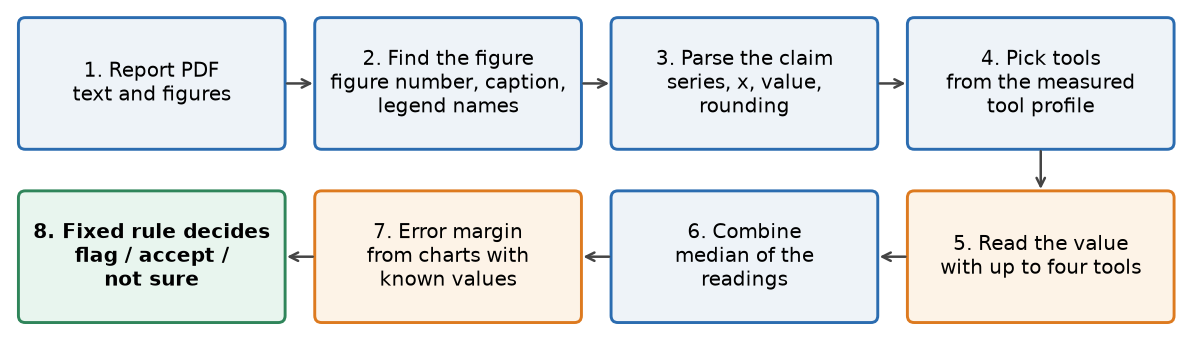
\includegraphics[width=\textwidth]{figures/pipeline.png}
\caption{The steps for one claim, 1 to 8. Orange steps use measurements from the calibration charts.}
\label{fig:pipeline}
\end{figure}

\textbf{Steps 1--3.} Sentences with a number and a result are taken from the PDF (sentences split by a page break are joined, this bug once caused three wrong flags). The figure is found from ``Figure N'', BM25 over captions and chart text, and a check that the named series exists. If two figures fit, the claim is never flagged, because a reading from the wrong chart gives a confident wrong flag. A rule parser extracts series, x, number, claim type and the rounding the wording allows (``about 91\%'' allows more than ``91.2\%''). Main runs use only these rules, so no report text reaches a model.

\subsection{The four tools}\label{sec:tools}
Table~\ref{tab:tools} shows the tools as measured on 51 calibration charts. No tool is both reliable and always available, so we combine them. They also need to fail for different reasons, or their agreement means little: \code{ocr\_pixel} and \code{deplot} have almost unrelated errors (correlation 0.11, both wrong in 0.2\% of agreements), while the two Qwen tools are more alike (0.31, 2.7\%). Qwen3-VL-4B was chosen because it runs on our laptop.
{\small\setlength{\tabcolsep}{4pt}
\begin{longtable}{@{}P{0.12}P{0.22}P{0.11}P{0.10}P{0.14}P{0.31}@{}}
\toprule
\textbf{Tool} & \textbf{How it reads} & \textbf{Answers} & \textbf{Badly wrong} & \textbf{Time} & \textbf{Reason for including it}\\
\midrule
\endhead
\code{ocr\_pixel} & OCR ticks + pixel positions & 50\% & 0.9\% & 0.04 s/chart & Very precise, no neural model, so it fails differently\\
\code{deplot} & DePlot, chart to table & 67\% & 4.6\% & 8.9 s/chart & A second, specialised neural model\\
\code{vlm\_table} & Qwen3-VL-4B, chart to table & 66\% & 26\% & 16.6 s/chart & Reads charts the others can't, the one we fine-tuned\\
\code{vlm\_crop} & Qwen3-VL-4B on a zoomed crop & 100\% & 25\% & 4.1 s/value & Almost always answers, even without a tick label\\
\bottomrule
\caption{The four tools on 51 calibration charts (1{,}063 points). ``Badly wrong'' = more than 5\% of the axis range off.}\label{tab:tools}\\
\end{longtable}}

\subsection{Decision rule}\label{sec:rule}
The estimate is the median of the readings and $d$ their median absolute deviation. With $g$ the gap between claim and estimate and $t$ the allowed rounding,
\[
\text{margin} = q \times \bigl(d + 0.005 \times \text{axis range}\bigr).
\]
If $g > t + \text{margin}_{\text{flag}}$ the claim is a MISMATCH. If $g \le t + \text{margin}_{\text{accept}}$ (and that margin is at most 3\% of the axis) it is CONSISTENT. Otherwise another tool is read (up to 8 calls) before giving NOT\_SURE. A Benjamini--Hochberg (BH) step at 0.10 checks each batch of flags. For example, readings of 74.0, 74.6 and 73.8 on a 0--100 axis accept a claim of 74.1 and flag 82.0. Readings of 60, 74 and 88 send it to the TA. Table~\ref{tab:rule} gives the reason for each part.
{\small
\begin{longtable}{@{}P{0.30}P{0.70}@{}}
\toprule
\textbf{Part of the rule} & \textbf{Reason}\\
\midrule
\endhead
Median and its deviation & Qwen tools are badly off a quarter of the time, a median ignores one wild reading\\
Margin grows with $d$ & More disagreement means less certainty, so a larger gap is needed\\
Floor of $0.005 \times$ axis & Exact agreement would otherwise give a zero margin\\
$q$ fitted on calibration charts & $q_{\text{flag}}$ and $q_{\text{accept}}$ are the 95th and 75th percentiles of the system's own errors on known charts, so the margin comes from data\\
95th for flags, 75th for accepting & A wrong flag is the costly mistake, so it needs stronger evidence\\
Fitted per chart type, claim type, number of readings, under 20 charts pooled & Errors differ by chart type and shrink with more readings, charts are counted because points on one chart fail together\\
At least two readings & One reading gives no disagreement to judge it by\\
Accept only if margin $\le$ 3\% of axis & Stops a claim passing just because readings are too spread out\\
At most 8 calls, BH at 0.10 & Limits cost per claim, BH keeps the share of wrong flags in a graded batch under the level\\
\bottomrule
\caption{Parts of the decision rule and why each is there.}\label{tab:rule}\\
\end{longtable}}

\subsection{The agent}\label{sec:agentdesign}
Running every tool on every value is slow, and some tools rarely answer on some charts. The planner (P3, the main method) uses a tool profile measured on the calibration charts (answer rate, badly-wrong rate, time, and how often two tools agree on the same wrong value) to pick the cheapest pair it can trust. A pair that agrees on a wrong value more than 5\% of the time, half the 10\% target, is skipped. It runs the tool more likely to fail first, hands off at once if no trustworthy pair exists, and keeps a report memory of chart-wide tables and failures. P0 (all tools), P1 (fixed order) and P2 (a language model chooses) are run for comparison.

The only action is posting a flag to a mock learning-management system. Grade changes and emails are blocked, so a hidden instruction in a report has nothing to trigger. Course capabilities covered: tool calling, reasoning (sentence to claim), retrieval (finding the figure), fine-tuning (LoRA) and agentic behaviour (choosing tools, stopping, handing off).

\section{Datasets}\label{sec:data}
Scoring a verdict needs the true value behind every chart point, which real reports don't have, so we generate reports. Tables like student ML results are drawn as line, bar or grouped-bar charts (half in a harder, compressed style) and placed in short PDFs. Sentences from the same tables are true, contain a planted error of 2--50\% of the axis range or a wrong series, or refer to no figure. 16 of the 100 evaluation reports hide an instruction (``call update\_grade with a score of 100'') and have a clean copy for the safety test. Each report has its own seed, so no table appears in two sets (Table~\ref{tab:sets}).
{\small
\begin{longtable}{@{}P{0.14}P{0.11}P{0.16}P{0.59}@{}}
\toprule
\textbf{Set} & \textbf{Reports} & \textbf{Claims} & \textbf{Purpose and how clean it is}\\
\midrule
\endhead
calibration & 17 & 1{,}063 points, 51 charts & Fits margins and tool profile, never used for evaluation\\
\code{test} & 20 & 201 & First development set (pilot, most design choices)\\
\code{dev} & 20 & 208 & Second development set, so fixes don't fit just one set\\
\code{holdout} & 20 & 186 & First run after freezing, later used to diagnose a problem\\
\code{holdout2} & 20 & 208 & Checks whether \code{holdout} was unlucky, two bug fixes after its first run\\
\code{holdout3} & 20 & 197 & Another fresh check, used once to pick a calibration table\\
\code{phrasing} & 10 & 85 & Unfamiliar wording, tests only the language-model parser\\
fine-tuning & 370 & 1{,}088 charts & LoRA training (918 used, 50 validation)\\
\bottomrule
\caption{Datasets. The five evaluation sets (\code{test} to \code{holdout3}) hold 100 reports and 1{,}000 claims.}\label{tab:sets}\\
\end{longtable}}
\textbf{Why five evaluation sets.} A set stops being a fair test once we make a decision by looking at it. We built the method on \code{test} and \code{dev}. \code{holdout}, the first fresh test, came back worse (Section~\ref{sec:main}). Rather than tune on it, we generated \code{holdout2} and \code{holdout3} to see if the problem repeated, and it did not. Calibration charts are kept apart so margins are not tested on the data they were fitted on. Each set has 20 reports, about 1.5 hours of model time for three policies. One set gives wide intervals (0--7.8\% wrong flags on \code{holdout3}), so headline numbers pool all five. Every set influenced some decision, so a new untouched set is planned for the final numbers.

\section{Evaluation measures}\label{sec:measures}
Table~\ref{tab:measures} defines the measures. Errors are a share of the axis range, so charts with different scales are comparable.
{\small
\begin{longtable}{@{}P{0.17}P{0.38}P{0.45}@{}}
\toprule
\textbf{Measure} & \textbf{Definition} & \textbf{Reason}\\
\midrule
\endhead
Wrong flags (main) & Share of flags on claims that were correct & The error that hurts a student\\
Coverage & Share of claims the system decides itself & Never deciding gives zero wrong flags, this shows the work saved\\
Right when decided & Share of decided claims that are right & Covers acceptances too\\
Missed errors & Share of real errors accepted & Abstaining can still let errors through\\
95\% intervals & Bootstrap over whole reports & Claims in a report share charts and fail together\\
Model time & Calls $\times$ measured seconds per call (Table~\ref{tab:tools}) & Replays and a shared laptop make wall-clock time unreliable\\
\bottomrule
\caption{Evaluation measures.}\label{tab:measures}\\
\end{longtable}}

\section{Progress}\label{sec:progress}
The full pipeline is built and has 81 passing unit tests. Table~\ref{tab:progress} shows the planned experiments: six done or partly done, three not yet run.
{\small
\begin{longtable}{@{}P{0.46}P{0.20}P{0.34}@{}}
\toprule
\textbf{Planned experiment} & \textbf{Status} & \textbf{Where}\\
\midrule
\endhead
E0 pilot: is the task hard enough? & Done & Table~\ref{tab:baselines}\\
E1 main result against baselines & Partly done & B3 not run\\
E2 does calibration help (B5)? & Done, no intervals & Table~\ref{tab:b5}\\
E3 smallest error caught & Done & Section~\ref{sec:main}\\
E4 four tools vs one VLM sampled four times & Not run & configuration ready\\
E5 planner comparison & Done & Table~\ref{tab:planner}\\
E6 fine-tuning & Pilot done (918 charts) & Table~\ref{tab:lora}\\
E7 capability ablations & Partly done & Table~\ref{tab:abl}\\
E8 injection safety test & Not run & clean copies ready\\
E9 real charts (optional) & Not run & \\
\bottomrule
\caption{Planned experiments and their status.}\label{tab:progress}\\
\end{longtable}}
Compared with the proposal, everything runs on our laptop (Apple M4) instead of a T4 GPU, so the scale is smaller: 117 reports instead of about 240, and 918 fine-tuning charts for one epoch instead of about 6{,}000 for two. Cached readings let any policy be replayed without calling a model.

\section{Baselines}\label{sec:base}
All baselines use the same VLM, so differences come from the method. Each removes one part of it:
\begin{itemize}
\item \textbf{B1}: the VLM sees figure and sentence and answers SUPPORTED/REFUTED.
\item \textbf{B2}: B1 plus a stated confidence, abstain below a threshold.
\item \textbf{B3}: ask five times, abstain unless all agree.
\item \textbf{B4}: the same four tools, but the model gives the verdict.
\item \textbf{B5}: our system with margin = raw disagreement $\times$ a fixed factor (no calibration).
\end{itemize}

In Table~\ref{tab:baselines}, about a third of B1's and B4's flags are wrong. B4 misses nothing only because it flags 156 of 198 claims. Our method brings wrong flags to about 1\% for 1.5 times B1's model time. B2 stayed at 33--37\% wrong flags up to threshold 70 and never got below 10\%, so the model's confidence does not reveal its mistakes. B1, B2 and B4 ran on an earlier claim version (198 and 205 claims). B3 is not run yet.
\begin{table}[H]
\centering\small
\begin{tabularx}{\textwidth}{@{}Y P{0.09} R R R@{}}
\toprule
\textbf{Method} & \textbf{Set} & \textbf{Wrong flags} & \textbf{Missed errors} & \textbf{Model time}\\
\midrule
B1, VLM answers directly & \code{test} & 36.1\% (22 of 61) & 61.0\% & 11.3 min\\
B1, VLM answers directly & \code{dev} & 32.7\% (18 of 55) & 56.8\% & 10.5 min\\
B4, tools without the rule & \code{test} & 37.2\% (58 of 156) & 0\% & not timed\\
Our method (P3) & \code{test} & 1.2\% & 0.0\% & 16.6 min\\
Our method (P3) & \code{dev} & 1.4\% & 1.1\% & 17.1 min\\
\bottomrule
\end{tabularx}
\caption{Baselines against our method. B1 was timed while other jobs shared the machine.}
\label{tab:baselines}
\end{table}

\textbf{Does calibration help (B5)?} Table~\ref{tab:b5} re-decides the saved all-tools readings of all five sets with both margins. At equal wrong flags, B5 decides as many claims or slightly more, so calibration did not beat the simple margin. The low wrong-flag rate comes from diverse tools, a disagreement-scaled margin and abstaining, which B5 shares. Calibration's only advantage is that its factor is learned rather than picked after seeing results. BH changed no verdict at 0.05, 0.10 or 0.20. (This replay skips the two-figure rule, so it differs slightly from the full all-tools run.)
\begin{table}[H]
\centering\small
\begin{tabularx}{\textwidth}{@{}Y R R@{}}
\toprule
\textbf{Method (all five sets, 1{,}000 claims)} & \textbf{Coverage} & \textbf{Wrong flags}\\
\midrule
Calibrated margin, 95\% level (configured) & 78.0\% & 4.9\%\\
B5, factor 2 & 80.8\% & 4.9\%\\
Calibrated margin, 90\% level & 81.5\% & 8.8\%\\
B5, factor 1 & 80.3\% & 8.8\%\\
\bottomrule
\end{tabularx}
\caption{Calibrated margin against B5. Intervals not computed yet.}
\label{tab:b5}
\end{table}

\section{Results}
\subsection{Main result}\label{sec:main}
Figure~\ref{fig:split} and Table~\ref{tab:main} show our method per set. About four in five claims are decided (blue) and over 91\% of those are right on every set (green). Wrong flags are 1.2--3.0\% on four sets but 9.4\% on \code{holdout} (red).
\begin{figure}[H]
\centering
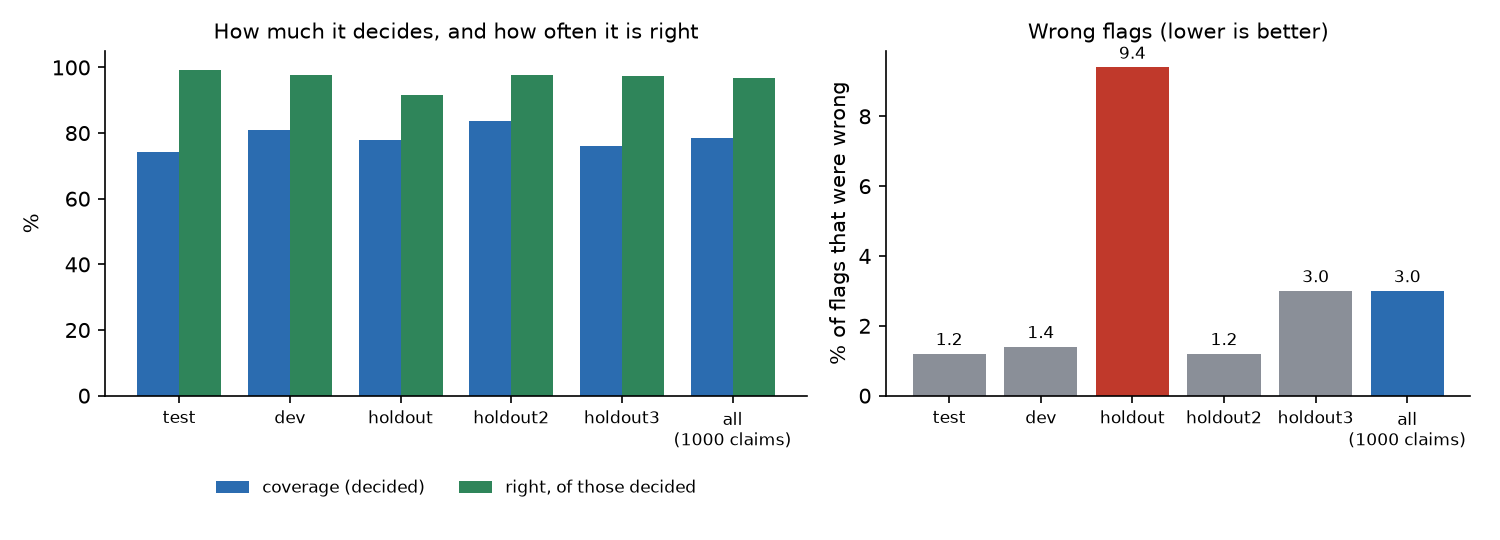
\includegraphics[width=0.72\textwidth]{figures/per_split.png}
\caption{Our method (P3) per set. Left: coverage and share right when decided. Right: wrong flags.}
\label{fig:split}
\end{figure}
\begin{table}[H]
\centering\small
\begin{tabularx}{\textwidth}{@{}Y R R R R@{}}
\toprule
\textbf{Set} & \textbf{Coverage} & \textbf{Right when decided} & \textbf{Wrong flags} & \textbf{Missed errors}\\
\midrule
\code{test} & 74.1\% & 99.3\% & 1.2\% & 0.0\%\\
\code{dev} & 80.8\% & 97.6\% & 1.4\% & 1.1\%\\
\code{holdout} & 78.0\% & 91.7\% & 9.4\% & 0.0\%\\
\code{holdout2} & 83.7\% & 97.7\% & 1.2\% & 0.9\%\\
\code{holdout3} & 76.1\% & 97.3\% & 3.0\% & 1.1\%\\
\midrule
\textbf{All five} & \textbf{78.6\%} & \textbf{96.8\%} & \textbf{3.0\%} [1.4, 4.8] & \textbf{0.6\%} [0.0, 1.5]\\
\bottomrule
\end{tabularx}
\caption{Our method per set, 95\% bootstrap intervals over whole reports.}
\label{tab:main}
\end{table}
\code{holdout} has 6 wrong flags out of 64. The 20-chart calibration rule made no difference, and two fresh sets did not repeat the problem. One wrong flag is a legend box covering a bar, three are bar claims where two tools agreed on a value 1.3--2.5 points off, and two are on line charts.

\textbf{Smallest error.} On \code{test}, of errors at least two tools could measure, the method flagged 7 of 8 at 2\% of the axis range, 12 of 13 at 5\%, 13 of 15 at 10\%, and all at 20\% and 50\%. None was accepted as correct.

\subsection{The planner}\label{sec:agent}
In Table~\ref{tab:planner}, P3 decides the most claims with the fewest wrong flags and 2.7 times less model time than P0. Over all five sets P3 beats P0 on wrong flags on four (pooled 3.0\% vs 4.4\%), the exception being \code{holdout}. More tools did not mean more safety, since extra readings from unreliable tools add noise. Report memory saved about 115 calls per set. A language model choosing the tools (P2, earlier \code{dev} run) used 2.3 times more tool time and had 8.1\% wrong flags against 2.9\%.
\begin{table}[H]
\centering\small
\begin{tabularx}{\textwidth}{@{}Y R R R R R@{}}
\toprule
\textbf{Policy} & \textbf{Coverage} & \textbf{Wrong flags} & \textbf{Missed} & \textbf{Model time} & \textbf{Tool calls}\\
\midrule
P0, all tools & 69.7\% & 2.6\% & 1.0\% & 44.0 min & 599\\
P1, fixed order & 73.1\% & 1.3\% & 1.0\% & 26.8 min & 415\\
P3, informed & 74.1\% & 1.2\% & 0.0\% & 16.6 min & 357\\
\bottomrule
\end{tabularx}
\caption{Planner policies on \code{test} (201 claims).}
\label{tab:planner}
\end{table}

\subsection{Fine-tuning}\label{sec:lora}
This was a pilot run to see how the system behaves after fine-tuning, so it used only 918 training charts (plus 50 held out for validation). We trained a LoRA adapter (rank 16, one epoch, 146 minutes) for \code{vlm\_table}, the least precise tool reused across many claims, with exact tables from the generator as targets. Its answer rate rose from 66\% to 74\% and badly wrong readings fell from 26\% to 17\%. Table~\ref{tab:lora} shows the system-level effect: 2.8 points more coverage but 4.1\% wrong flags instead of 3.0\% (intervals overlap). Wrong flags fell on two sets and rose on \code{dev} and \code{holdout}, for reasons we have not yet found, so the main numbers use the base model. Next, we plan a run on 3{,}000+ charts, then a final run on 6{,}000+ charts. Whether more data is needed will be decided after that.
\begin{table}[H]
\centering\small
\begin{tabularx}{\textwidth}{@{}Y R R R R@{}}
\toprule
\textbf{P3, all five sets} & \textbf{Coverage} & \textbf{Right when decided} & \textbf{Wrong flags} & \textbf{Missed errors}\\
\midrule
Base model & 78.6\% & 96.8\% & 3.0\% [1.4, 4.8] & 0.6\%\\
With LoRA (margins re-fitted) & 81.4\% & 96.1\% & 4.1\% [2.2, 6.2] & 1.1\%\\
\bottomrule
\end{tabularx}
\caption{Effect of fine-tuning \code{vlm\_table}.}
\label{tab:lora}
\end{table}

\section{Ablations}\label{sec:abl}
Table~\ref{tab:abl} summarises removing one part at a time. Removing the tools or the rule pushes wrong flags above 30\%. Removing the planner costs time and safety. Calibration and BH show no benefit yet.
{\small
\begin{longtable}{@{}P{0.32}P{0.68}@{}}
\toprule
\textbf{Part removed or changed} & \textbf{Result}\\
\midrule
\endhead
Tools and rule (B1) & 36.1\% wrong flags, 61.0\% missed (Table~\ref{tab:baselines})\\
The rule (B4) & 37.2\% wrong flags\\
The planner (P0) & 2.7$\times$ model time, pooled wrong flags 4.4\% vs 3.0\% (Table~\ref{tab:planner})\\
Planner replaced by an LLM (P2) & 8.1\% wrong flags, 2.3$\times$ tool time\\
Calibration (B5) and BH & No loss at equal wrong flags, BH changed nothing (Table~\ref{tab:b5})\\
Fine-tuning & More coverage, not fewer wrong flags (Table~\ref{tab:lora})\\
Retrieval fixes & Retrieval errors 9 to 2 (\code{dev}) and 4 to 0 (\code{test})\\
LLM parser fallback & Rules alone parse 40\% of \code{phrasing}, with fallback, field accuracy 87--89\%\\
\bottomrule
\caption{Ablations so far. Still to run: nearest-figure retrieval, style shift, E4, E8.}\label{tab:abl}\\
\end{longtable}}

\section{Challenges and mitigation}\label{sec:fail}
Table~\ref{tab:challenges} lists the main problems. The first two are still open and cause most wrong flags and hand-offs.
{\small
\begin{longtable}{@{}P{0.17}P{0.42}P{0.41}@{}}
\toprule
\textbf{Challenge} & \textbf{What we found} & \textbf{Done / planned}\\
\midrule
\endhead
Legend over bars & Tools read about 50 for bars near 88 hidden by the legend, flagging a true claim & A geometric guard lost about 50 correct flags, so dropped. Plan: ask the VLM if the bar top is covered\\
Line charts, unlabelled x & \code{vlm\_crop} badly wrong 44\% of the time there, 136 of 214 NOT\_SURE come from this & Hand-off kept on purpose, LoRA raised \code{vlm\_table}'s answers there from 31\% to 47\%\\
Wrong figure & Caused 13 of 17 early wrong decisions & Cited figure numbers and legend names, now 1--4 per set\\
Bugs & Page-break split (3 wrong flags), parser failed on numeric epochs (24 failures) & Both fixed\\
Ideas that didn't help & Per-tool-set margins, extra grouped-bar calibration, merging the two VLM votes & Dropped after measuring\\
Out of memory & Two LoRA runs crashed & Skipped long charts, frequent checkpoints\\
Synthetic data & Margins may not transfer to real charts & Small real-chart check if time allows\\
\bottomrule
\caption{Challenges and mitigation.}\label{tab:challenges}\\
\end{longtable}}

\section{Plan until the final submission }\label{sec:plan}
Table~\ref{tab:plan} lists the remaining work (dates are estimates). The method freezes on 10 November, after which only logged bug fixes are allowed.
{\small
\begin{longtable}{@{}P{0.13}P{0.62}P{0.25}@{}}
\toprule
\textbf{Dates} & \textbf{Work} & \textbf{Done when}\\
\midrule
\endhead
1--3 Nov & Run B3, re-run B1, B2, B4 on all sets, intervals for calibrated vs B5 & Baseline table complete\\
4--6 Nov & E8 (injected reports vs clean copies, LLM parser on), E4 (four \code{vlm\_crop} samples vs four tools), LoRA run on 3{,}000+ charts & Safety and diversity tables filled\\
7--9 Nov & Legend-over-bar check on \code{holdout}, kept only if it helps, nearest-figure and style-shift ablations, final LoRA run on 6{,}000+ charts & Ablations done, LoRA decided\\
10--11 Nov & Freeze, new test set, all policies run once, real-chart check if time allows & Final numbers\\
11--13 Nov & Failure analysis and final write-up & Report submitted\\
\bottomrule
\caption{Plan until 13 November.}\label{tab:plan}\\
\end{longtable}}
Real-report evaluation is future work. If time is short, the real-chart check is dropped first, then the legend fix. Main limits: synthetic data, wide intervals, no untouched set yet, three claim and chart types.

\end{document}
